\chapter{Introdução}

O interesse em fontes alternativas de energia é relativamente recente e vem crescendo rapidamente. Entre outras razões para esse interesse podemos citar o sistemático aumento no preço dos combustíveis fósseis e da energia elétrica. O impacto ambiental envolvido na produção e consumo destas fontes de energia, na forma dos gases de efeito estufa, também não pode ser ignorado. Uma dessas alternativas é o uso de lixo orgânico e rejeito animal para a produção de biogás.

O processo de produção de biogás a partir de resíduos orgânicos e dejeto animal já é conhecido há muito tempo (FERRAZ, 1980). O biogás gerado desta forma é composto por aproximadamente 60\% de gás metano (CH4) e 38\% de dióxido de carbono (CO2). A mistura gasosa obtida, por ser rica em metano, pode ser utilizada como combustível. Além disso, os resíduos da produção de biogás podem ser utilizados como adubo. O equipamento utilizado para a produção de biogás é chamado de biodigestor.

O presente relatório tem como objetivo checar a viabilidade técnica e econômica da construção e utilização de biodigestores em pequena escala, utilizando-se biodigestores de batelada compactos e construídos a partir de materiais simples e baratos. 

\section{Problemas e objetivos}

A investigação da viabilidade da construção e utilização de biodigestores em pequena escala pretende melhorar o entendimento da tecnologia envolvida na produção do biogás e tem como principais objetivos:

\begin{itemize}
\item Investigar os custos envolvidos na construção de um biodigestor;
\item Identificar a matéria prima utilizada na produção de biogás;
\item Quantificar a produção de biogás por unidade de matéria prima;
\item Verificar os possíveis problemas advindos da utilização de um biodigestor.
\end{itemize}

De acordo com Ferraz (1980, p. 20), biodigestores com 2 metros cúbicos são capazes de gerar 1100 litros de biogás por dia. A proposta deste presente relatório é verificar se há possibilidade de se construir um biodigestor ainda menor. Com menos de 1 metro cúbico de volume.

\section{Justificativa}

Com o aumento no custo da energia, é cada vez mais importante pesquisar novas fontes energéticas, de preferência fontes limpas e renováveis. A geração de biogás é barata pois usa como matéria prima o lixo orgânico e resíduos animais. Além disso, até mesmo os resíduos da produção do biogás podem ser reaproveitados.

Contudo, é necessário investigar mais a fundo a viabilidade técnica e econômica da produção de biogás em pequena escala por meio do uso de um biodigestor. 

Finalmente, é importante lembrar que o Brasil recebeu, ainda na década de 70, com a crise do petróleo, a tecnologia da digestão anaeróbica (PECORA, 2006). Portanto, a tecnologia já é bem conhecida, o que ajuda a diminuir os riscos.

\section{Consumo energético no estado de São Paulo}

No gráfico abaixo podemos verificar o consumo anual de energia elétrica e de petróleo no estado de São Paulo desde o ano de 2006 até 2017. A partir destes dados foi criada uma previsão baseada em uma tendência linear até o ano de 2025. De acordo com estas informações, o consumo anual de energia elétrica pode passar dos atuais 129.810.078 MWh para 151.885.615 MWh, um aumento significativo de 17\%. Já no caso do petróleo, o consumo pode aumentar 26\%, passando dos atuais 29.337 milhões de litros para 37.126 milhões de litros (SECRETARIA DE INFRAESTRUTURA E MEIO AMBIENTE DO ESTADO DE SÃO PAULO, 2018).

\vspace{0.8cm}

\begin{figure}[htb]
	\begin{center}
	    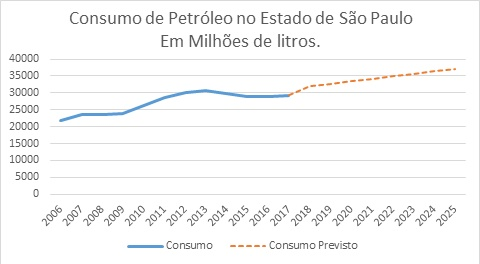
\includegraphics[scale=1.0]{consumo_petroleo_sp.jpg}
	\end{center}
	\vspace*{-0.5cm}
	\caption{\label{fig_grafico}Consumo de petróleo no estado de São Paulo}
	%\legend{Fonte: \citeonline[p. 24]{araujo2012}}
\end{figure}

\begin{figure}[htb]
	\begin{center}
	    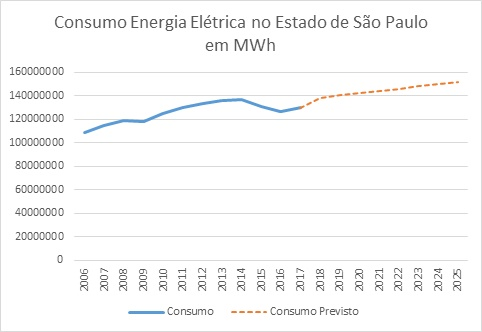
\includegraphics[scale=1.0]{consumo_eletricidade_sp.jpg}
	\end{center}
	\vspace*{-0.5cm}
	\caption{\label{fig_grafico}Consumo de de eletricidade no estado de São Paulo}
	%\legend{Fonte: \citeonline[p. 24]{araujo2012}}
\end{figure}

